\newpage
\section{Tool di conversione}
\label{sez:tc}

In questa sezione viene presentato il tool in grado di convertire il file .xmi estratto con Modelio, in un file adatto all'utilizzo del tool di verifica automatica VerifPal.\\
La scelta di creare un file utilizzabile da VerifPal è motivata dal fatto che è più semplice e intuitivo riuscire a trovare delle relazioni tra il file .xmi e i blocchi che compongono il modello del protocollo nel linguaggio di questo tool rispetto al linguaggio Applied Pi Calculus utilizzato da ProVerif.\\
Il tool si può scomporre in due parti, nella prima si occupa di generare un file intermedio, a partire dal file .xmi, contenente delle strutture in grado di rappresentare le relazioni tra i blocchi e le InformationFlow della modellazione tramite UML.\\ 
Mentre nella seconda parte viene utilizzato il file intermedio generato nella prima parte per andare a generare un template, il quale consente al progettista di inserire il tipo dell'attaccante (attivo o passivo) e quali sono le verifiche che vuole effettuare sul protocollo nel blocco di queries, prima di utilizzare il file come input a VerifPal.\\
La Figura \ref{fig:p1} rappresenta la modellazione della prima parte del tool attraverso un flowchart, possiamo vedere come dato il file .xmi come input, il tool trasformi l'input in un albero in modo da poterlo navigare ed estrarne le informazioni rilevanti.\\
Partendo dalla radice il tool estrae i vari tipi degli oggetti istanziati nel modello UML, tra i vari tipi troviamo InputPort, OutPort, FunctionalBlock, FunctionalArchitecture, InformationFlow.\\
Dopo aver estratto i tipi il tool si occupa di verificare se sono presenti degli oggetti di tipo Node, di solito utilizzati per la rappresentazione fisica dei dispositivi.\\ 
Nel caso in cui sia presente un oggetto di tipo Node naviga i suoi attributi per estrarre le informazioni sugli oggetti che lo compongono, nello specifico estrae id, nome e tipo dell'oggetto che compone l'oggetto di tipo Node e salva queste informazioni in un dizionario.\\
Il passo successivo del tool è quello di vedere se vi sono oggetti di tipo Instance, in questo caso, come per gli oggetti che compongono il Node, estrae id, nome e tipo dell'oggetto e li salva nello stesso dizionario.\\
Infine il tool cerca le InformationFlow, per ognuna di queste salva in un dizionario id dell'oggetto sorgente, id dell'oggetto destinazione e le informazioni sul messaggio.\\
La particolarità del dizionario per le InformationFlow è che oltre alle informazioni estratte viene mantenuto anche un contatore, il contatore sarà utile nella seconda parte del tool per mantenere l'ordine dell'interazione tra gli agenti partecipanti al protocollo.\\
Una volta terminata la costruzione dei dizionari il tool si occupa di andarli a scrivere sul file che verrà utilizzato nella seconda parte.\\
\begin{figure}[h!] 
    \centering 
    \fbox{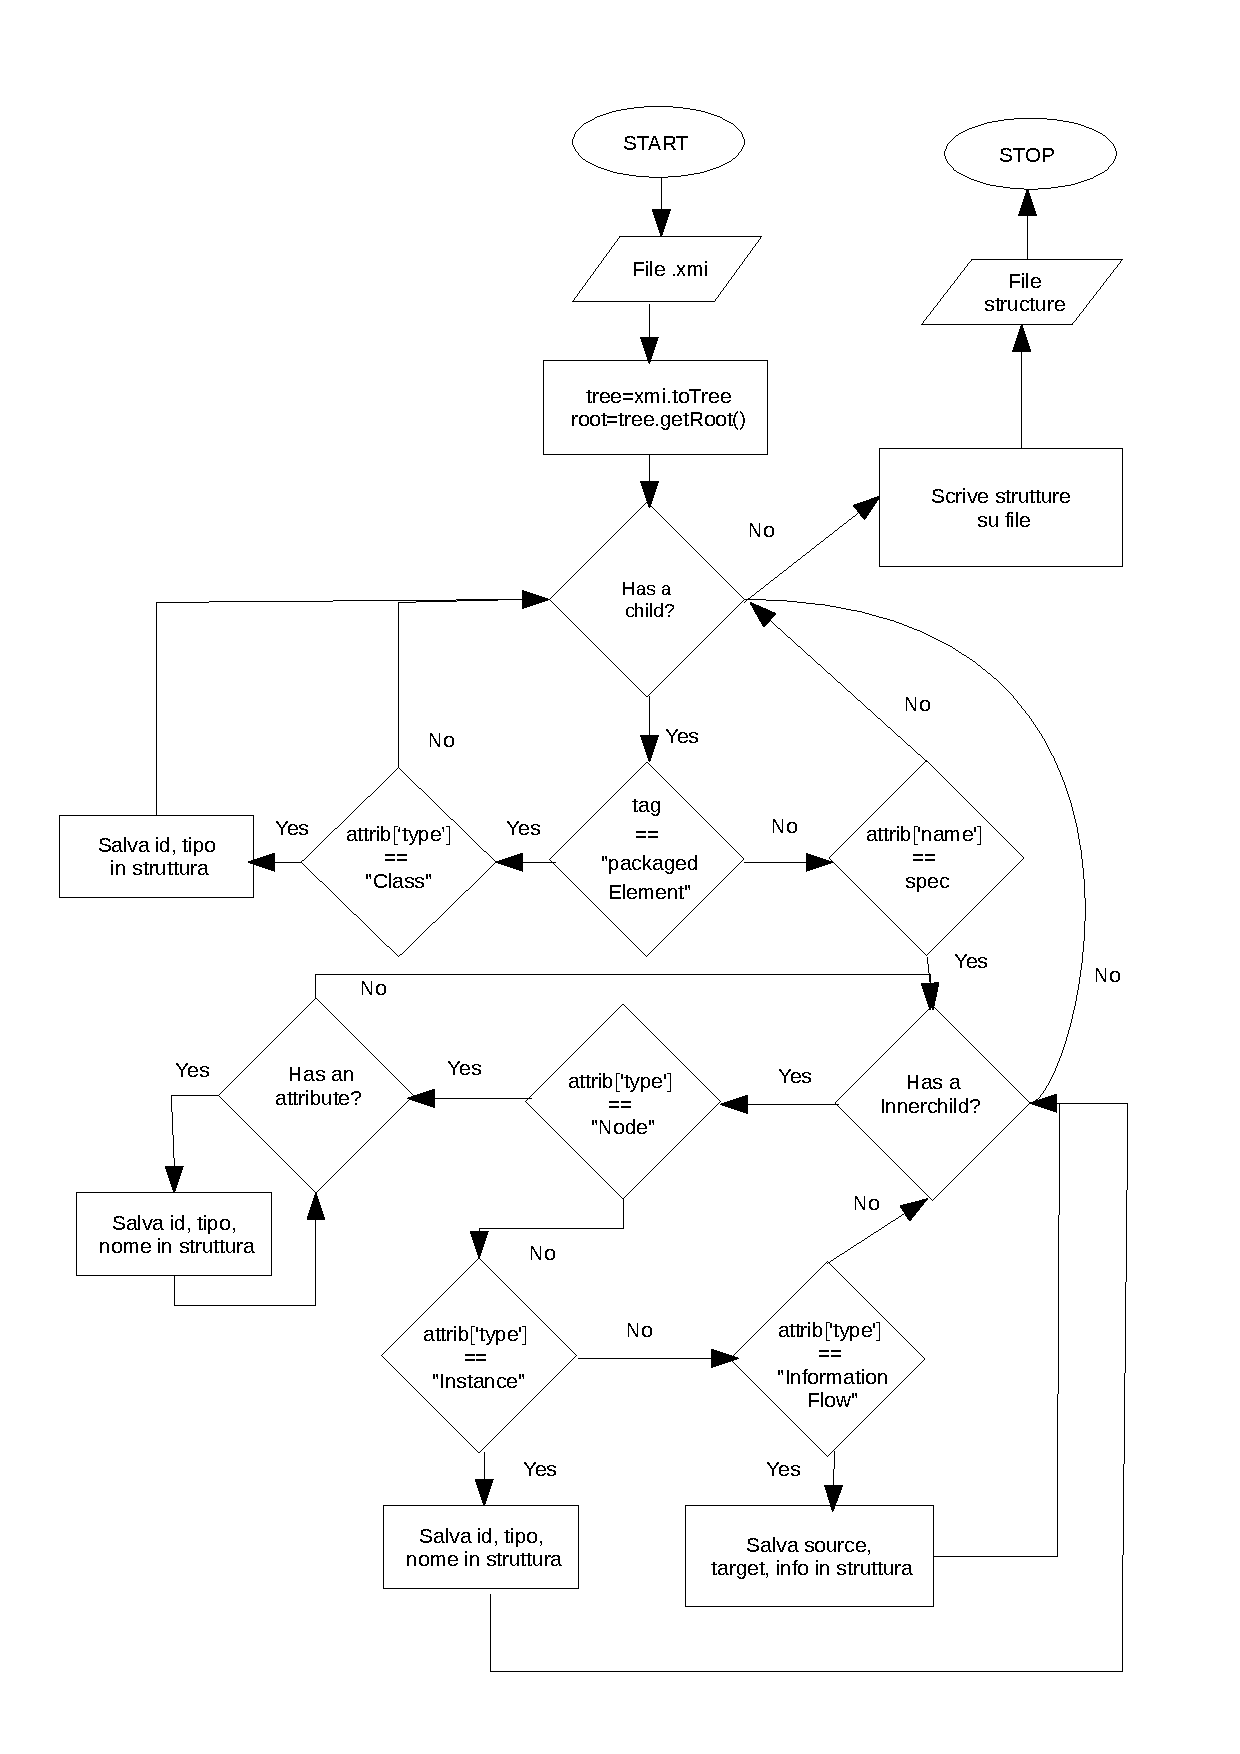
\includegraphics[width=\textwidth]{../img/parser_1.pdf}}
    \caption{Flowchart modellazione prima parte del tool}
    \label{fig:p1} 
\end{figure}
\clearpage
\noindent Nella Figura \ref{fig:exex} è rappresentata l'estrazione dei dizionari dell'esempio di modellazione UML in Figura \ref{fig:exUML}.\\
\begin{figure} [h!]
    \lstinputlisting[basicstyle=\footnotesize, frame=single,breaklines= true]{../code/output/ex_struct.txt}
    \caption{Esempio di estrazione delle strutture da parte del tool}
    \label{fig:exex}
\end{figure}
\\
\noindent La figura \ref{fig:p2} rappresenta la modellazione tramite flowchart della seconda parte del tool, dove dato in input il file contenente le strutture viene restituito il template per VerifPal.\\
Il funzionamento della seconda parte del protocollo consiste nello scorrere il dizionario delle InformationFlow, per ogni elemento nel dizionario si utilizza l'id della destinazione per verificare nel dizionario degli oggetti se la destinazione è di tipo OutputPort, in questo caso il tool si trova di fronte ad un invio di messaggio ad un secondo principal, questo viene convertito nella stringa adatta \texttt{A -> B : messaggio}.\\
Nel caso in cui l'oggetto di destinazione non sia una porta di output significa che le informazioni dell'InformationFlow sono un input per un FunctionalBlock, si utilizza il nome dell'oggetto per mapparlo in una primitiva di VerifPal e passargli le varie informazioni come argomenti.\\ 
Per mappare i nomi degli oggetti con le primitive all'interno del tool è presente un dizionario che mappa le primitive di VerifPal con i nomi degli oggetti.\\
Questo tipo di mappatura tra nomi e primitive richiede una standardizzazione dei nomi degli oggetti che deve essere fatta in fase di modellazione dei diagrammi UML. \\
La standardizzazione consiste nel definire dei blocchi di oggetti standard, che rappresentano le primitive, i quali devono semplicemente essere utilizzati dal progettista, in modo che non sia lui stesso a crearli con dei nomi che non trovano riscontro all'interno del dizionario di mappatura utilizzato dal tool.\\
A livello di creazione del template si può dire che tutti gli oggetti di tipo InformationFlow, compresi tra due InformationFlow con destinazione oggetti di tipo OutputPort, corrispondono alle operazioni fatte da un principal.\\
Quando il tool si trova di fronte ad oggetti che hanno solo informazioni in uscita, si trova di fronte a blocchi in cui le informazioni possono essere conoscenze pregresse del pricipal oppure informazioni generate al momento, in questo caso è in grado di distinguere se deve utilizzare la parola chiave \texttt{knows} oppure \texttt{generates}.  
\newpage 
\begin{figure}[h!] 
    \centering 
    \fbox{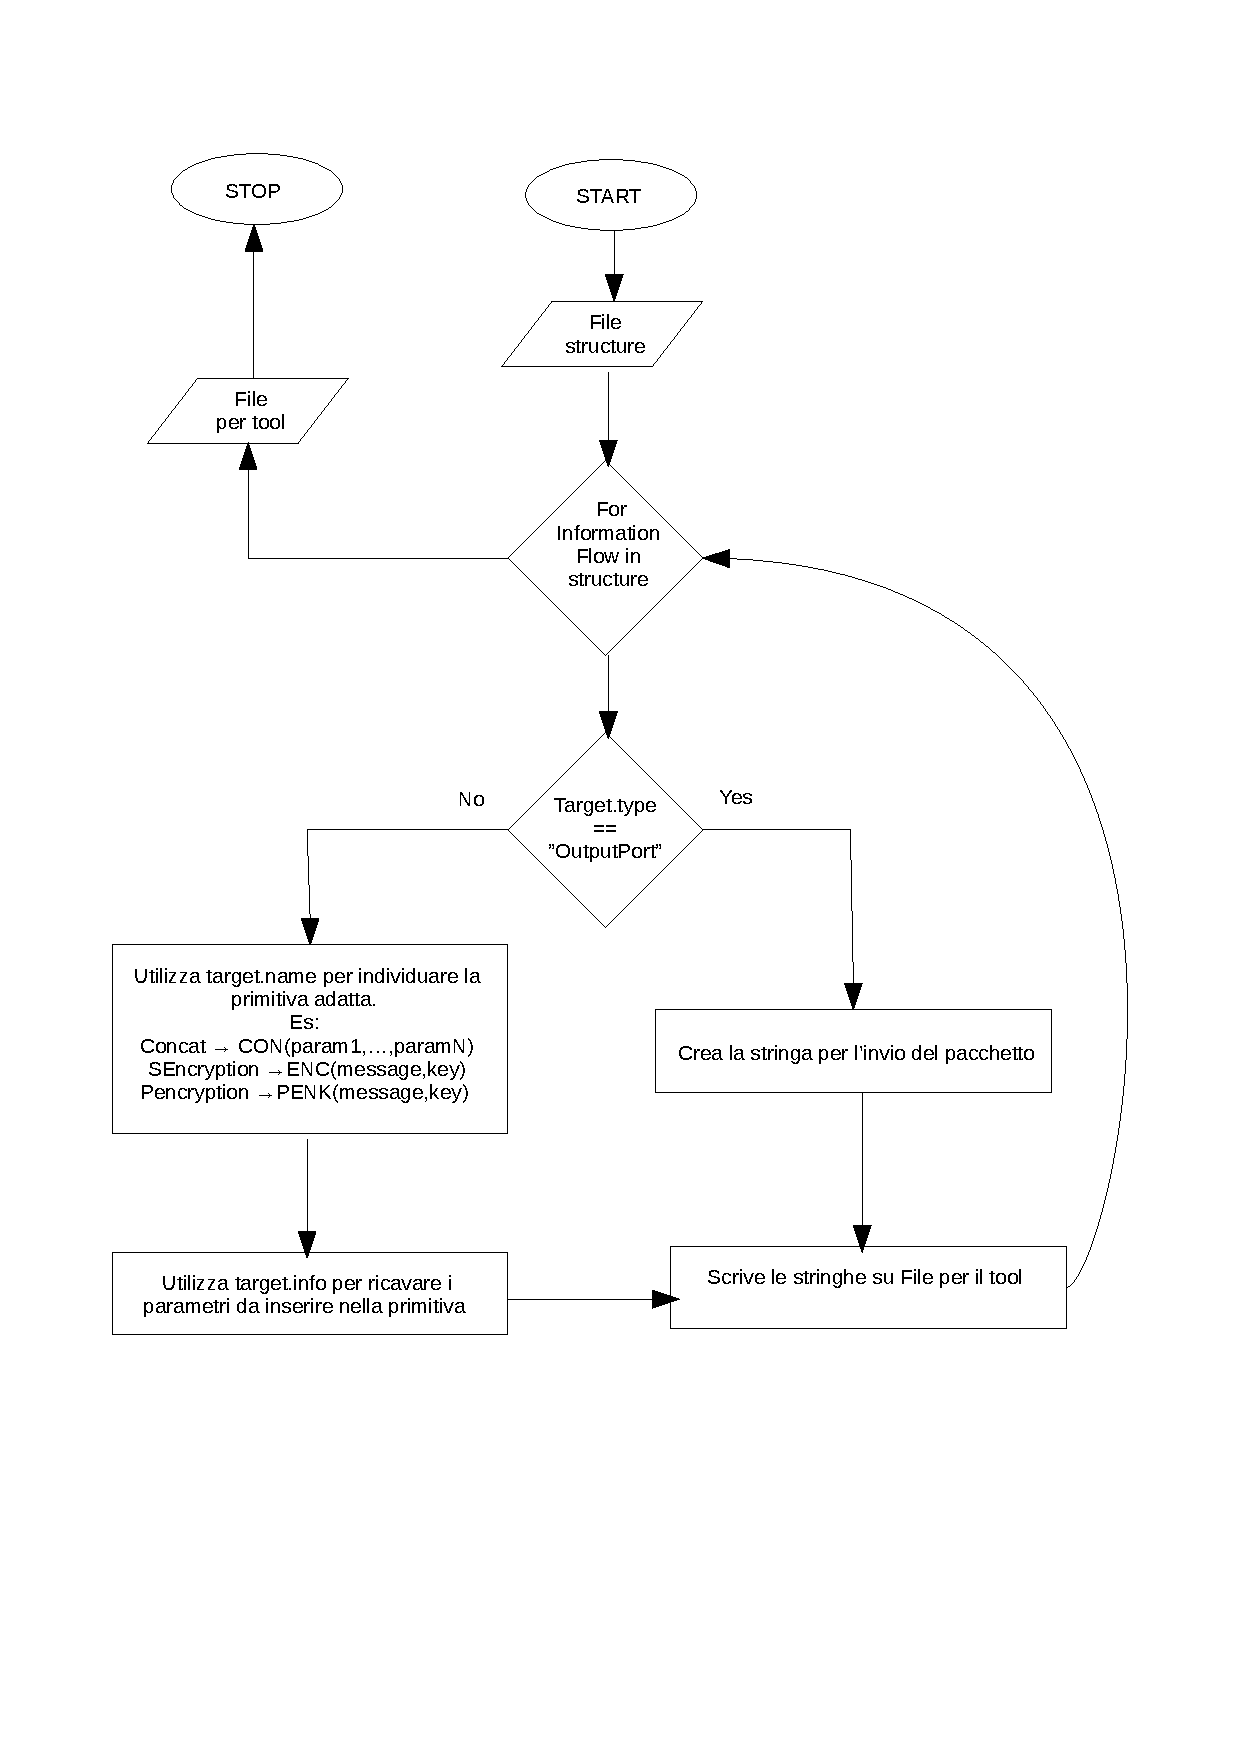
\includegraphics[width=\textwidth]{../img/parser_2.pdf}}
    \caption{Flowchart modellazione seconda parte del tool}
    \label{fig:p2} 
\end{figure}
\clearpage
\begin{figure}[h!] 
    \lstinputlisting[language=vp]{../code/verifpal/ex.vp}
    \caption{Esempio di template per VerifPal}
    \label{fig:extem} 
\end{figure}
\noindent In Figura \ref{fig:extem} vediamo il template ottenuto nella seconda parte del tool partendo dal file delle strutture descritto in Figura \ref{fig:exex}.
